\chapter{Multimodal UNet with Early Fusion}
\label{ch:early_fusion_model}
Following the single-modality baseline, this chapter introduces a more advanced approach using a multimodal UNet. This model leverages the principle of \textbf{early fusion} to combine two complementary perfusion maps - Cerebral Blood Flow (CBF) and Time to Maximum (Tmax) - to improve the accuracy and robustness of lesion segmentation.

\section{Early Fusion Explained}
\label{sec:early_fusion_explained}
Early fusion, also known as data-level or input-level fusion, is a strategy in multimodal deep learning where information from different sources is combined at the very beginning of the modeling pipeline. In the context of medical imaging, this involves stacking different image modalities as separate channels of a single input tensor before they are fed into the neural network's first layer.

The process is analogous to h ow a standard color image is represented by stacking red, green, and blue (RGB) channels. For our 3D UNet, instead of a single-channel input, we create a multi-channel tensor where, for example, the first channel corresponds to the CBF map and the second to the Tmax map. The network then learns to extract and integrate features from this combined representation from the outset. This approach allows the model to identify complex, inter-modal relationships at the earliest and deepest levels of its architecture.



\section{Implementation and Modality Selection}
\label{sec:implementation_fusion}
The transition from a single-modality to a multimodal model required careful consideration of which modalities to combine and specific adaptations to the MONAI pipeline.

\subsection{Rationale for Modality Selection}
\label{subsec:modality_rationale} 
The decision to use \textbf{CBF and Tmax} and to deliberately exclude CTA was driven by two considerations: creating a clear contrast to the CTA only baseline and exploiting their complementary information. As both modalities were introduced earlier in the report, we do not repeat their definitions here. In short, combining magnitude- and delay-based perfusion cues provides a more complete physiological signal and is expected to better separate ischemic core from surrounding tissue, improving segmentation performance.

\subsection{Adaptations to the MONAI Pipeline}
\label{subsec:pipeline_adaptations}
Implementing the early fusion model required several key modifications to the existing pipeline:

\begin{itemize}
    \item \textbf{Data Loading:} The \texttt{LoadImaged} transform was configured to load multiple image keys (e.g., \verb|keys=['cbf', 'tmax', 'label']|) for each case. The data loading logic was also made more robust to ensure that a case was only included if all required modality files were present.
    
    \item \textbf{Intensity Scaling:} Unlike CTA, perfusion maps do not use Hounsfield Units. Therefore, a separate \texttt{ScaleIntensityRanged} transform was applied to normalize the perfusion maps to a [0, 1] range based on typical physiological values, rather than a specific window and level.

    \item \textbf{The Fusion Step:} The core of the implementation is the \texttt{ConcatItemsd} transform. After individual loading and scaling, this transform stacks the CBF and Tmax tensors along the channel dimension, creating a new, single item named "image" with a shape of \verb|[2, H, W, D]|. This fused tensor serves as the input for all subsequent augmentations and for the model itself.

    \item \textbf{Model Architecture:} The \texttt{UNet} instantiation was adapted to accept the new input shape by setting its \verb|in_channels| parameter to the number of modalities being fused (i.e., \verb|in_channels=2|). The rest of the network's architecture, including its depth and channel configuration, remained consistent with the first model to ensure a fair comparison.
\end{itemize}


\section{Results and Comparative Analysis}
\label{sec:results_comparison}
The multimodal model, trained on Fold 1, demonstrated a significant improvement over the single-modality baseline. Its best performance resulted in a Dice coefficient of 0.172 and a 95th percentile Hausdorff Distance of 41.1 mm.

\subsection{Comparative Analysis with Single-Modality Model}
\label{subsec:comparative_analysis}
A direct comparison of the training progression reveals the profound impact of the multimodal approach. Figure~\ref{fig:performance_comparison} plots the key evaluation metrics for both models over the first 24 epochs.

\begin{figure}[htbp]
    \centering
    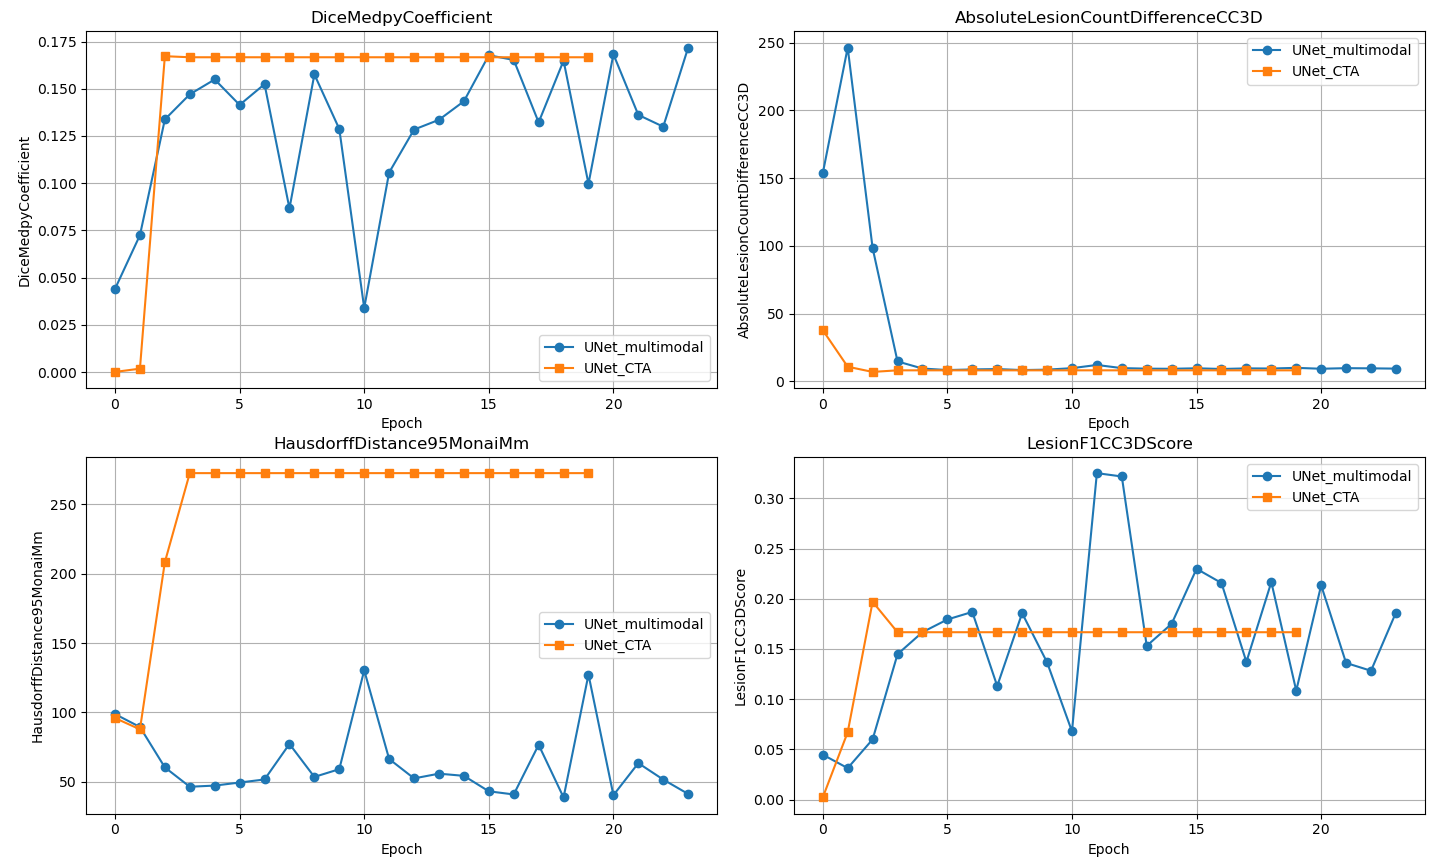
\includegraphics[width=\textwidth]{figures/compare_plot.png}
    \caption{Comparative performance analysis of the multimodal (CBF\_TMAX) and single-modality (CTA) models across four key metrics. The plots illustrate the learning progression during the initial 24 epochs of training.}
    \label{fig:performance_comparison}
\end{figure}

The analysis of these results highlights two critical findings:

\begin{itemize}
    \item \textbf{Training Stability and Learning:} The multimodal model exhibits a clear, albeit noisy, learning curve. All metrics show a general trend of improvement after an initial difficult phase. In strong contrast, the CTA model's training appears to have collapsed after the third epoch. Its metrics become completely static, indicating that the model converged to a trivial and incorrect local minimum, rendering its results unreliable.

    \item \textbf{Peak Performance and Boundary Accuracy:} The multimodal model not only shows a successful training process but also achieves superior performance. It reached a higher peak Dice coefficient and, most importantly, a vastly better 95th percentile Hausdorff Distance (41.1 mm vs. a stuck 272.6 mm). This indicates that the predictions from the fusion model align much more closely with the ground truth boundaries, a direct result of the richer input data allowing it to learn more meaningful anatomical features. The lower Absolute Lesion Count Difference further suggests it is better at identifying the correct number of lesions.
\end{itemize}

In conclusion, the early fusion of CBF and Tmax proved to be a far more effective strategy than relying on CTA alone. The complementary information provided by the perfusion maps enabled the model to overcome the challenges of class imbalance and feature ambiguity that likely caused the single-modality model to fail.